%%%%%%%%%%%%%%%%%%%%%%%%%%%%%%%%%%%%%%%%%%%%%%%%%%%%%%%%
\documentclass[12pt,a4paper]{article}% 文档格式
\usepackage{ctex,hyperref}% 输出汉字
\usepackage{times}% 英文使用Times New Roman
%%%%%%%%%%%%%%%%%%%%%%%%%%%%%%%%%%%%%%%%%%%%%%%%%%%%%%%%
\title{\fontsize{18pt}{27pt}\selectfont% 小四字号,1.5倍行距
	{\heiti% 黑体 
		凸优化在支持向量机的应用}}% 题目
%%%%%%%%%%%%%%%%%%%%%%%%%%%%%%%%%%%%%%%%%%%%%%%%%%%%%%%%
%\author{\fontsize{12pt}{18pt}\selectfont% 小四字号,1.5倍行距
	%	{\fangsong% 仿宋
		%		Evildoer}
	%	\fontsize{10.5pt}{15.75pt}\selectfont% 五号字号,1.5倍行距
	%	{\fangsong% 仿宋
		%		()}}% 作者单位,“~”表示空格
%%%%%%%%%%%%%%%%%%%%%%%%%%%%%%%%%%%%%%%%%%%%%%%%%%%%%%%%
\date{}% 日期(这里避免生成日期)
%%%%%%%%%%%%%%%%%%%%%%%%%%%%%%%%%%%%%%%%%%%%%%%%%%%%%%%%
\usepackage{amsmath,amsfonts,amssymb}% 为公式输入创造条件的宏包
%%%%%%%%%%%%%%%%%%%%%%%%%%%%%%%%%%%%%%%%%%%%%%%%%%%%%%%%
\usepackage{graphicx}% 图片插入宏包
\usepackage{subfigure}% 并排子图
\usepackage{float}% 浮动环境,用于调整图片位置
\usepackage[export]{adjustbox}% 防止过宽的图片
%%%%%%%%%%%%%%%%%%%%%%%%%%%%%%%%%%%%%%%%%%%%%%%%%%%%%%%%
\usepackage{bibentry}
\usepackage{natbib}% 以上2个为参考文献宏包
%%%%%%%%%%%%%%%%%%%%%%%%%%%%%%%%%%%%%%%%%%%%%%%%%%%%%%%%
\usepackage{abstract}% 两栏文档,一栏摘要及关键字宏包
%\renewcommand{\abstracttextfont}{\fangsong}% 摘要内容字体为仿宋
%\renewcommand{\abstractname}{\textbf{摘\quad 要}}% 更改摘要二字的样式
%%%%%%%%%%%%%%%%%%%%%%%%%%%%%%%%%%%%%%%%%%%%%%%%%%%%%%%%
\usepackage{xcolor}% 字体颜色宏包
\newcommand{\red}[1]{\textcolor[rgb]{1.00,0.00,0.00}{#1}}
\newcommand{\blue}[1]{\textcolor[rgb]{0.00,0.00,1.00}{#1}}
\newcommand{\green}[1]{\textcolor[rgb]{0.00,1.00,0.00}{#1}}
\newcommand{\darkblue}[1]
{\textcolor[rgb]{0.00,0.00,0.50}{#1}}
\newcommand{\darkgreen}[1]
{\textcolor[rgb]{0.00,0.37,0.00}{#1}}
\newcommand{\darkred}[1]{\textcolor[rgb]{0.60,0.00,0.00}{#1}}
\newcommand{\brown}[1]{\textcolor[rgb]{0.50,0.30,0.00}{#1}}
\newcommand{\purple}[1]{\textcolor[rgb]{0.50,0.00,0.50}{#1}}% 为使用方便而编辑的新指令
%%%%%%%%%%%%%%%%%%%%%%%%%%%%%%%%%%%%%%%%%%%%%%%%%%%%%%%%
\usepackage{url}% 超链接
\usepackage{bm}% 加粗部分公式
\usepackage{multirow}
\usepackage{booktabs}
\usepackage{epstopdf}
\usepackage{epsfig}
\usepackage{longtable}% 长表格
\usepackage{supertabular}% 跨页表格
\usepackage{algorithm}
\usepackage{algorithmic}
\usepackage{changepage}% 换页
%%%%%%%%%%%%%%%%%%%%%%%%%%%%%%%%%%%%%%%%%%%%%%%%%%%%%%%%
\usepackage{enumerate}% 短编号
\usepackage{caption}% 设置标题
\captionsetup[figure]{name=\fontsize{10pt}{15pt}\selectfont 图}% 设置图片编号头
\captionsetup[table]{name=\fontsize{10pt}{15pt}\selectfont Table}% 设置表格编号头
%%%%%%%%%%%%%%%%%%%%%%%%%%%%%%%%%%%%%%%%%%%%%%%%%%%%%%%%
\usepackage{indentfirst}% 中文首行缩进
\usepackage[left=2.50cm,right=2.50cm,top=2.80cm,bottom=2.50cm]{geometry}% 页边距设置
\renewcommand{\baselinestretch}{1.5}% 定义行间距(1.5)
\renewcommand{\abstractname}{\textbf{\large {摘\quad 要}}} %更改摘要二字的样式
%%%%%%%%%%%%%%%%%%%%%%%%%%%%%%%%%%%%%%%%%%%%%%%%%%%%%%%%
\usepackage{fancyhdr} %设置全文页眉、页脚的格式
\pagestyle{fancy}
\hypersetup{colorlinks=true,linkcolor=black}% 去除引用红框,改变颜色
%%%%%%%%%%%%%%%%%%%%%%%%%%%%%%%%%%%%%%%%%%%%%%%%%%%%%%%%







\begin{document}% 以下为正文内容
	\maketitle% 产生标题,没有它无法显示标题
	%%%%%%%%%%%%%%%%%%%%%%%%%%%%%%%%%%%%%%%%%%%%%%%%%%%%%%%%
	\lhead{}% 页眉左边设为空
	\chead{}% 页眉中间设为空
	\rhead{}% 页眉右边设为空
	\lfoot{}% 页脚左边设为空
	\cfoot{\thepage}% 页脚中间显示页码
	\rfoot{}% 页脚右边设为空
	%%%%%%%%%%%%%%%%%%%%%%%%%%%%%%%%%%%%%%%%%%%%%%%%%%%%%%%%
	%	\begin{abstract}
		%		\fangsong 为了以后能摆大烂而创造了一个模板,为了展现转行效果而开始啊对对对对对对对对对对对对对对对
		%	\end{abstract}
	%	
	%	\begin{adjustwidth}{1.06cm}{1.06cm}
		%		\fontsize{10.5pt}{15.75pt}\selectfont{\heiti{关键词:}\fangsong{摆大烂、啊对对对}}\\
		%	\end{adjustwidth}

	\begin{center}% 居中处理
		
		\author{ 控制一班 谢硕 }
		
		\date{2023/1/9}
		
		
		
		{\textbf{摘要}}% 英文摘要
	\end{center}
	\begin{adjustwidth}{1.06cm}{1.06cm}% 英文摘要内容
		\hspace{1.5em}支持向量机(SVM)是一种基于统计学习理论的机器学习方法,由于其优越的学习性能,已经成为当前模式识别、数据挖掘等机器学习领域的研究热点。本文对于支持向量机理论进行了推导,以深刻体会凸优化理论在支持向量机理论中的应用,并加强自己对凸优化的理解。
		
	\end{adjustwidth}
	\begin{center}
		\large{\textbf{Abstract}}
	\end{center}
	
	\begin{adjustwidth}{1cm}{1cm}
		\hspace{1.5em}Support vector machine (SVM) is a machine learning method based on statistical learning theory, which has become a research hotspot in the field of machine learning such as pattern recognition and data mining due to its superior learning performance. This paper derives the theory of support vector machines to deeply appreciate the application of convex optimization theory in support vector machine theory and strengthen my own understanding of convex optimization.
	\end{adjustwidth}
	\thispagestyle{empty}       %本页不显示页码
	\newpage
	\begin{center}
	\tableofcontents	
	\end{center}

	\thispagestyle{empty}       %本页不显示页码
	\newpage% 从新的一页继续
	\setcounter{page}{1}        %从下面开始编页,页脚格式为导言部分设置的格式

	
	
	\section{凸优化理论在线性可分支持向量机的应用}
	\subsection{问题描述}
	设有数目不同的8个学生团体,按单位坐成8个学生团体,按单位坐成8个圆团,利用四条直线$g_1(x)$,$g_2(x)$,$g_3(x)$,$g_4(x)$,把它们按如图1(a)、(b)所示的形式分隔开,我们要找出哪几个团队之间的分隔线最合理。
	通过观察相邻团队到分隔线的间距,易看出图1中的团队一与二、六与七、七与八的分隔间距较大相对合理,而图2中相邻两个团队之间的分隔间距都较大,因此都比较合理。
	\begin{figure}[htbp]
		\begin{minipage}[t]{0.5\linewidth}
			\centering
			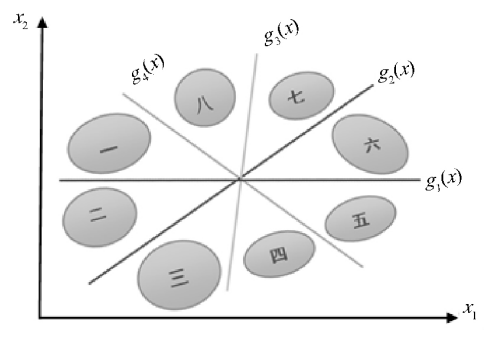
\includegraphics[width=\textwidth]{figure1}
			\centerline{\fontsize{10pt}{15pt}(a) 团队间任意分隔}
		\end{minipage}%
		\begin{minipage}[t]{0.5\linewidth}
			\centering
			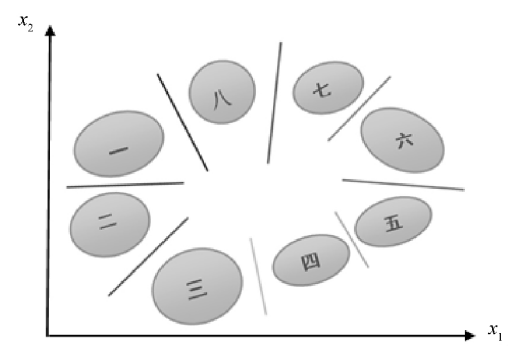
\includegraphics[width=\textwidth]{figure2}
			\centerline{\fontsize{10pt}{15pt}(b) 团队间最佳分隔}
		\end{minipage}
		\caption{\fontsize{10pt}{15pt}团队间分隔方式}
	\end{figure}
	
	\subsection{点到直线$l$的距离$d$}
	对于如图2所示的直线$l:{x}_{2}=k{x}_{1}+b$,可以变形为$k{x}_{1}-{x}_{2}+b=0$。为了方便,写成向量形式,令$x={({x}_{1},{x}_{2})}^{T}$,则直线$l$可写成$g(x)=(k,-1){({x}_{1}),{x}_{2}}^{T}+b={w}^{T}x+b=w·x+b=0$。
	
	\begin{figure}[H]% 插入一张图片,H表示浮动环境下的here
		\centering
		\begin{minipage}{0.6\textwidth}% 小页面尺寸,可自行调节
			\centering
			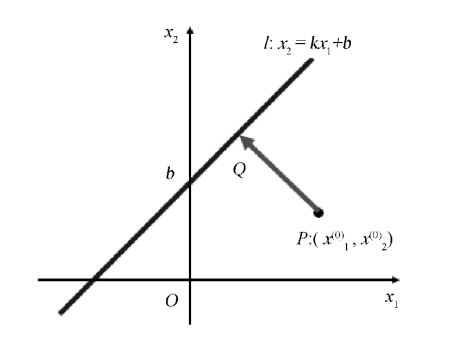
\includegraphics[width=0.8% 图片尺寸,可自行调节
			\textwidth]{figure3}% 图片名称(图片需与tex文件在同一文件夹)
			\caption{\fontsize{10pt}{15pt}\selectfont 点到直线的距离}% 图例
		\end{minipage}
	\end{figure}
	从上可知,改变$w$和$b$的数值,可分别确定直线的方向和位置,它是确定最佳分类线的基础。由初等数学知,点$P({{x}_{1}^{0}},{{y}_{2}^{0}})$到直线$l$的距离为
	\begin{align}
		d=\dfrac{\left|k{{x}_{1}}^{(0)}-{{x}_{2}}^{(0)}+b\right|}{ \sqrt{{k}^{2}+{(-1)}^{2}}}=\dfrac{\left|{w}^{T}{x}^{(0)}+b \right|}{\left\|w\right\|}
	\end{align}
	如图3,当两直线${l}_{1}:{x}_{2}={k}_{1}{x}_{1}+{b}_{1}$和${l}_{2}:{x}_{2}={k}_{2}{x}_{1}+{b}_{2}$平行时。有${k}_{1}={k}_{2}$,只有${b}_{1}$和${b}_{2}$不同,所以有平行直线间的距离为
	\begin{align}
		d=\dfrac{\left|{b}_{1}-{b}_{2}\right|}{\sqrt{{k}^{2}+{(-1)}^{2}}}=\dfrac{\left|{b}_{1}-{b}_{2}\right|}{\left\|w\right\|}
	\end{align}
	\begin{figure}[H]% 插入一张图片,H表示浮动环境下的here
		\centering
		\begin{minipage}{0.6\textwidth}% 小页面尺寸,可自行调节
			\centering
			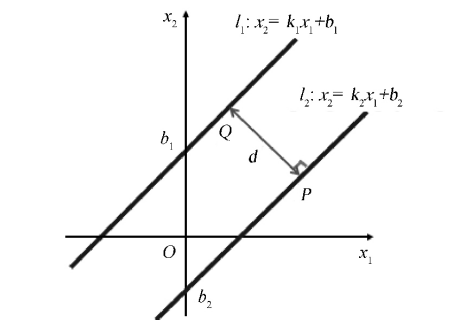
\includegraphics[width=0.8% 图片尺寸,可自行调节
			\textwidth]{figure4}% 图片名称(图片需与tex文件在同一文件夹)
			\caption{\fontsize{10pt}{15pt}\selectfont 平行线间的距离}% 图例
		\end{minipage}
	\end{figure}
	
	\subsection{将$d$引入支持向量机(SVM)}
	所谓SVM,就是寻找一条分类线,使之到两类样本中最近点的距离最大的一种机器学习算法。对图4(a),要用一条直线,将图中的实心点和空心点分开,显然,图上的这条直线就是一条分类线,而由于图4(b)的分隔线显然分类效果更好,因为其分类间隔更宽。
	
	\begin{figure}[htbp]
		\begin{minipage}[t]{0.5\linewidth}
			\centering
			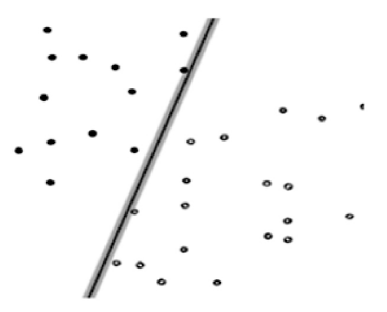
\includegraphics[width=\textwidth]{figure5}
			\centerline{\fontsize{10pt}{15pt}(a) 任意分隔线}
		\end{minipage}%
		\begin{minipage}[t]{0.5\linewidth}
			\centering
			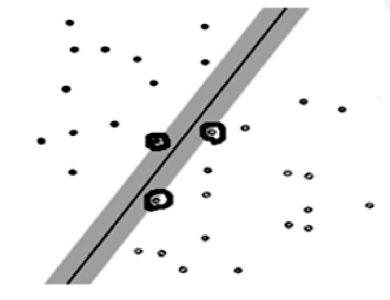
\includegraphics[width=\textwidth]{figure6}
			\centerline{\fontsize{10pt}{15pt}(b) 最佳分隔线}
		\end{minipage}
		\caption{\fontsize{10pt}{15pt}寻找一条分类线}
	\end{figure}
	而对图5,已知实心、空心两类共$L$个训练样本${\left\{\left({x}^{(i)},{y}^{(i)} \right) \right\}}_{i=1}^{L}$,样本特征${x}^{i}={\left({x}_1^{(i)},{x}_2^{(i)}\right)}$,样本分类值为${y}^{(i)}{\in}{\left\{-1,1\right\}} $。
	\begin{figure}[H]% 插入一张图片,H表示浮动环境下的here
		\centering
		\begin{minipage}{0.83\textwidth}% 小页面尺寸,可自行调节
			\centering
			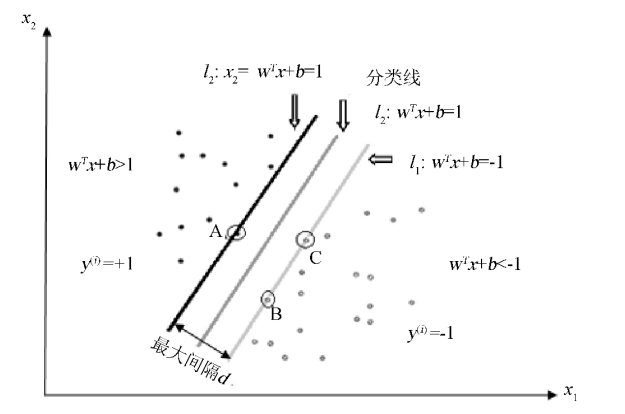
\includegraphics[width=0.8% 图片尺寸,可自行调节
			\textwidth]{figure7}% 图片名称(图片需与tex文件在同一文件夹)
			\caption{\fontsize{10pt}{15pt}\selectfont SVM分类图}% 图例
		\end{minipage}
	\end{figure}
	设分类先为$l:g(x)={w}^{T}x+b=0$,$l$右下侧的线为${l}_{1}:g(x)={w}^{T}x+b=-1$,$l$左上侧的线为${l}_{2}:g(x)={w}^{T}x+b=1$。则离分类线$l$最近的样本$x$满足$\left|g(x)=1\right|$(即在面${l}_{1}$或${l}_{2}$上),这样的$x$称为支持向量。把分类值${y}^{(i)}$考虑进去,两类样本点满足的统一表达式为${({w}^{T}{x}^{(i)}+b){y}^{(i)}\geq1}$,$i=1,2,···,L$。这时${l}^{1}$与${l}^{2}$之间的距离为:$d=\frac{2}{||w||}$。
	为了能把两类样本分得更开,就希望在满足${({w}^{T}{x}^{(i)}+b){y}^{(i)}\geq1}$,$i=1,2,···,L$的条件下,$d=\frac{2}{||w||}$最大,这显然是一个条件极值问题。
	\subsection{条件极值的求法}
	求解上面的问题,即求$d=\frac{2}{||w||}$在约束条件${({w}^{T}{x}^{(i)}+b){y}^{(i)}\geq1}$,$i=1,2,···,L$下的最大值。求法如下:
	
	步骤1: 将约束条件写成${({w}^{T}{x}^{(i)}+b){y}^{(i)}-1\geq0}$,$i=1,2,···,L$;
	
	步骤2: 为了便于计算,将求$d=\frac{2}{||w||}$最大,转化为求$\frac{1}{2}{||w||}^{2}$最小。
	
	步骤3:
	利用拉格朗日函数求极值,设拉格朗日函数为:
	\begin{align}
		L(w,b,a)=\frac{1}{2}{||w||}^{2}-\sum_{i=1}^{L} {\alpha}_{i}\left[{({w}^{T}{x}^{(i)}+b){y}^{(i)}-1}\right]
	\end{align}
	其中,Lagrange系数${\alpha}_{i}\geq0$,$i=1,2,···,L,\alpha={({\alpha}_{1},{\alpha}_{1},···,{\alpha}_{L})}^{T}$。
	
	步骤4:
	对(3)式分别关于w和b求偏导数,并令它们等于零,得
	\begin{align}
		\begin{cases} \frac{\partial{L(w,b,\alpha)}}{\partial{w}_{k}}={w}_{k}-\sum_{i=1}^{L}  {\alpha _{i}{y}^{(i)}{x}_k^{i}=0,k=1,2,···,n}\\ \frac{\partial{L(w,b,\alpha)}}{\partial{b}}=\sum_{i=1}^{L}{{\alpha }_{i}{y}^{(i)}=0,k=1,2,···,n} \\ \end{cases} 
	\end{align}
	即
	\begin{align}
		\begin{cases} w=\sum_{i=1}^{L} {\alpha }_{i}{y}^{(i)}{x}^{(i)}\\ \sum_{i=1}^{L} {\alpha_{i}{y}^{(i)}=0}\\ \end{cases} 
	\end{align}
	
	步骤5:
	把第(3)式展开,再将(5)式的等量关系代入,就变成
	\begin{align}
		L(w,b,\alpha)=\frac{1}{2}{||w||}^{2}-\sum_{i=1}^{L} {\alpha}_{i}\left[{y}^{(i)}{({w}^{T}{x}^{(i)}+b)}-1\right]
	\end{align}
	\begin{align}
		=\frac{1}{2}{||w||}^{2}-{w}^{T}\sum_{i=1}^{L} {\alpha }_{i}{y}^{(i)}{x}^{(i)}-b\sum_{i=1}^{L} {\alpha }_{i}{y}^{(i)}+\sum_{i=1}^{L} {\alpha}^{i}
	\end{align}
	\begin{align}
		=\sum_{i=1}^{L} {\alpha}^{i}-\frac{1}{2}{\left(\sum_{i=1}^{L} {\alpha }_{i}{y}^{(i)}{x}^{(i)} \right)}^{T}\left(\sum_{i=1}^{L} {\alpha }_{i}{y}^{(i)}{x}^{(i)} \right)=Q(\alpha)
	\end{align}
	
	要求$Q(\alpha)$在边界约束${\alpha}_{i}\geq0$,$i=1,2,···,L$和等式约束$\sum_{i=1}^{L} {\alpha }_{i}{y}^{(i)}=0$下的最值点。
	显然,$Q(\alpha)$是关于$\alpha$的二次函数,这是一个在凸集约束下的优化问题,且具有上面的边界约束和线性等式约束.求解该问题的标准形式为
	\begin{align}
		\begin{cases} min f(\alpha)=-Q(\alpha)=\frac{1}{2}{\alpha}^{T}H{\alpha}+{C}^{T}\alpha    \\ s.t.\quad	{A}_{eq}^{T}\alpha=0\\
			{	\qquad	} lb\leq\alpha \\ \end{cases} 
	\end{align}
	
	其中,$M=\left[{x}^{(1)},{x}^{(2)},···,{x}^{(L)}\right]×\left[ \begin{array}{cccc}   %该矩阵一共3列,每一列都居中放置
		{y}^{(1)} & \quad & \quad & \quad\\  %第一行元素
		\quad & {y}^{(2)} & \quad & \quad\\  %第二行元素
		\quad & \quad & · & \quad  \\  %第二行元素
		\quad & \quad & · & {y}^{(L)}  \\  %第二行元素
	\end{array} 
	\right]$,$H={M}^{T}M$,$C={[-1,-1,···,-1]}^{T}$,${A}_{eq}={[{y}^{(1)},{y}^{(2)},···,{y}^{(L)}]}^{T}$,$lb={[0,0,···,0]}^{T}$。
	如图6所示,可以直观的理解二次二次凸函数在唯一凹点${\alpha}^{*}$处取到最小值(最优解)。
	\begin{figure}[H]% 插入一张图片,H表示浮动环境下的here
		\centering
		\begin{minipage}{0.6\textwidth}% 小页面尺寸,可自行调节
			\centering
			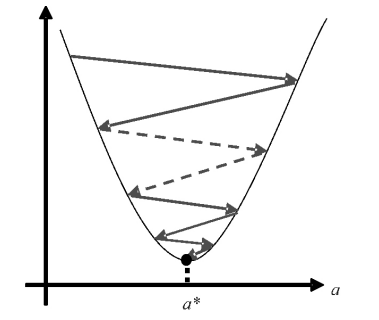
\includegraphics[width=0.8% 图片尺寸,可自行调节
			\textwidth]{figure8}% 图片名称(图片需与tex文件在同一文件夹)
			\caption{\fontsize{10pt}{15pt}\selectfont 二次凸函数的最值}% 图例
		\end{minipage}
	\end{figure}
	
	对于该问题,则可利用Matlab中专门求解二次规划问题的quadprog函数,如下式
	\begin{align}
		\begin{cases} min f(x)=-\frac{1}{2}{x}^{T}H{x}+{c}^{T}x   \\ 
			s.t.\quad	Ax\leq b\\
			\qquad {A}_{eq}x={b}_{eq}    \\
			\qquad lb\leq x \leq ub\\\end{cases} 
	\end{align}
	
	其中,$x=quadprog(H,c,A,b,{A}_{eq},{b}_{eq},lb,ub,{x}_{0},options)$。针对本问题,可求出唯一全局最优解${\alpha}^{*}$,且这个优化问题的解是在边界条件上取得,即满足
	\begin{align}
		{\alpha}_{i}\left[{y}^{(i)}{({w}^{T}{x}^{(i)}+b)}-1\right]=0,i=1,2,···,L
	\end{align}	
	
	则\textcircled{1}当${y}^{(i)}{({w}^{T}{x}^{(i)}+b)}-1>0$时,必有${\alpha}_{i}=0$;
	
	\textcircled{2}当${\alpha}_{i}>0$时,必有${y}^{(i)}{({w}^{T}{x}^{(i)}+b)}-1>0$时,必有${\alpha}_{i}=0$。说明${x}^{(i)}$是支持向量,它们通常只是占总样本中的很少一部份。
	
	只要求出$Q(\alpha)$的最值点${\alpha}^{*}$,则由式(5)就可得
	\begin{align}
		{w}^{*}=\sum_{i=1}^{L} {\alpha }_{i}^{*}{y}^{(i)}{x}^{(i)}
	\end{align}			
	
	再由式(1)的条件或式(11)选出的支持向量直接求得
	\begin{align}
		{b}^{*}=-\frac{\max\limits_{{y}_{i}=-1} {({w}^{*})}^{T}{x}^{(i)}+\max\limits_{{y}_{i}=-1}{({w}^{*})}^{T}{x}^{(i)}}{2}
	\end{align}		
	上式由根据离分类线最近的正的函数间隔等于离分类线最近的负的函数间隔所得。
	
	步骤6:
	从而得到最优分类线
	\begin{align}
		g(x)={({w}^{*})}^{T}x+{b}^{*}=\sum_{i=1}^{L} {\alpha}_{i}^{*}{y}^{(i)}({x}^{(i)}·x)+{b}^{*}=0
	\end{align}	
	
	则两类问题的分类函数为:
	\begin{align}
		{S}_{(x)}=sgn\left\{\sum_{i=1}^{L} {\alpha}_{i}^{*}{y}^{(i)}({x}^{(i)}·x)+{b}^{*}\right\}=	
		\begin{cases}  
			+1,when\sum_{i=1}^{L} {\alpha}_{i}^{*}{y}^{(i)}({x}^{(i)}·x)+{b}^{*}>0时;\\ 
			-1,when\sum_{i=1}^{L} {\alpha}_{i}^{*}{y}^{(i)}({x}^{(i)}·x)+{b}^{*}<0时;\\
			0,when\sum_{i=1}^{L} {\alpha}_{i}^{*}{y}^{(i)}({x}^{(i)}·x)+{b}^{*}=0时 \\ \end{cases} 
	\end{align}	
	
	综合上述方法,可得出如下的SVM分类步骤为:
	
	\textcircled{1}通过已知样本的特征${x}^{(i)}$和类别样本${y}^{(i)}(\pm1)$,求得最佳分类参数${\alpha}_{i}^{*}$和${b}^{*}$;
	
	\textcircled{2}将待判别的样本特征$x$代入分类函数式(15),就可得到分类结果。
	
	
	\section{凸优化理论在非线性可分支持向量机的应用}
	\subsection{问题引入}
	通过利用非线性模型才能很好地进行分类的问题称为非线性分类问题,如图7所示。两类数据分别分布为两个圆圈的形状,不论是任何高级的分类器,只要它是线性的,就没法处理,SVM也不行。因为这样的数据本身就是线性不可分的,是一个典型的非线性可分问题。
	\begin{figure}[H]% 插入一张图片,H表示浮动环境下的here
		\centering
		\begin{minipage}{0.6\textwidth}% 小页面尺寸,可自行调节
			\centering
			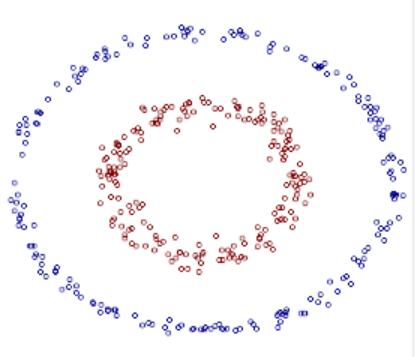
\includegraphics[width=0.8% 图片尺寸,可自行调节
			\textwidth]{figure9}% 图片名称(图片需与tex文件在同一文件夹)
			\caption{\fontsize{10pt}{15pt}\selectfont 典型的非线性可分问题}% 图例
		\end{minipage}
	\end{figure}
	非线性问题往往不好求解,所以我们希望用线性分类问题的方法来解决这个问题。所采用的方法是进行非线性变换。
	\subsection{核函数与核技巧}
	首先,核函数有如下定义。
	
	设$\chi$是输入空间,$\aleph$为特征空间,如果存在一个从$\chi$到$\aleph$的映射:
	\begin{align}
		\phi(x):\chi\rightarrow\aleph
	\end{align}
	
	使得对所有$x,z\in\chi$,函数$K(x,z)$满足条件:
	\begin{align}
		K(x,z)=\phi(x)·\phi(z)
	\end{align}
	则称$K(x,z)$为核函数,$\phi(x)$为映射函数,式中$\phi(x)·\phi(z)$为内积。
	
	常用的核函数有:
	
	线性核:
	\begin{align}
		K({x}_{i},{x}_{j})={x}_{i}^{T}{x}_{j}
	\end{align}
	
	多项式核:
	\begin{align}
		K({x}_{i},{x}_{j})={({x}_{i}^{T}{x}_{j})}^{p}  ,\qquad p\geq1
	\end{align}
	
	高斯核:
	\begin{align}
		K({x}_{i},{x}_{j})=exp(-\frac{{||{x}_{i}-{x}_{j}||}^{2}}{2{\sigma}^{2}}),\qquad\sigma>1
	\end{align}
	
	拉普拉斯核:
	\begin{align}
		K({x}_{i},{x}_{j})=exp(-\frac{||{x}_{i}-{x}_{j}||}{\sigma}),\qquad\sigma>0
	\end{align}
	
	线性分类方法求解非线性分类问题一般分为两步:\textcircled{1}使用一个变换将原空间的数据映射到新空间。\textcircled{2}在新空间里使用线性分类学习方法从训练数据中学习分类模型.核技巧就是属于上诉介绍的方法,应用到支持向量机的基本思想就是通过一个非线性变换将输入空间对应于一个特征空间,使得在输入空间中的超曲面模型对应于特征空间中的超平面模型。核技巧的思想为:在学习与预测中只定义核函数$K(x,z)$,而不显式地定义映射函数$\phi$.为通常计算$K(x,z)$比较容易,而通过$\phi(x)$和$\phi(z)$的内积来计算$K(x,z)$并不容易。$\phi$是输入空间到特征空间的映射,特征空间$\aleph$往往是高维的,甚至是无穷维。且对于给定的核$K(x,z)$,特征空间$\aleph$和映射函数$\phi$的取法并不唯一。
	
	对于线性可支持向量机,无论是目标函数还是决策函数(分离超平面)都只涉及输入实例与实例之间的内积。在对偶问题的目标函数中的内积${x}_{i}$,${x}_{j}$,可以用核函数$K(x,z)=\phi(x)·\phi(z)$来代替。此时对偶问题的目标函数成为:
	\begin{align}
		W(\alpha)=\frac{1}{2}\sum_{i=1}^{N} {\sum_{j=1}^{N} {{\alpha}_{i}{\alpha}_{j}{y}_{i}{y}_{j}K({x}_{i},{x}_{j})}}-\sum_{i=1}^{N} {\alpha}_{i}
	\end{align}
	分类决策函数变为:
	\begin{align}
		{S}_{(x)}=sgn\left\{\sum_{i=1}^{{N}_{S}} {\alpha}_{i}^{*}{y}^{(i)}K(x,{x}_{i})+{b}^{*}\right\}
	\end{align}
	这就等价于:经过映射函数$\phi$将原来的输入空间变换到一个新的特征空间,将输入空间中的内积${x}_{i}·{x}_{j}$变换为特征空间中的内积$\phi({x}_{i})·\phi({x}_{j})$,在新的特征空间里,从训练样本中学习线性支持向量机,当映射函数是非线性函数时,学习到的含有核函数的支持向量机是非线性模型。在核函数$K(x,z)$给定的条件下,可以利用求解线性分类问题的方法求解非线性分类问题的支持向量机。学习是隐式地在特征空间进行,不需要显式地定义特征空间和映射函数,这样的技巧称为核技巧。
	\subsection{非线性支持向量机学习算法}
	假设输入训练数据集为:$T=\left\{({x}_{1},{y}_{1}),({x}_{2},{y}_{2}),···,({x}_{N},{y}_{N}) \right\}$,其中,${x}_{i}\in\chi={R}^{n},{y}_{i}\in y=\left\{-1,+1\right\},i=1,2,···,N;$输出为分类决策函数。具体算法步骤如下:
	
	步骤1:
	选取适当的核函数$K(x,z)$和适当的参数$C$,构造并求解如下优化问题:
	\begin{align}
		\begin{cases} \min\limits_{\alpha} \frac{1}{2} 
			\sum_{i=1}^{N} {\sum_{j=1}^{N} {{\alpha}_{i}{\alpha}_{j}{y}_{i}{y}_{j}K({x}_{i},{x}_{j})}}-\sum_{i=1}^{N} {\alpha}_{i} \\ s.t.\quad	\sum_{i=1}^{N} {{\alpha}_{i}{y}_{i}}=0\\
			{	\qquad	} 0\leq{\alpha}_{i}\leq C,i=1,2,···,N \\ \end{cases} 
	\end{align}
	求得最优解${\alpha}^{*}=({\alpha}_{1}^{*},{\alpha}_{2}^{*},···, {\alpha}_{N}^{*})$
	
	步骤2:
	选择${\alpha}^{*}$的一个正分量$0<{\alpha}_{j}<{C}$,计算:
	\begin{align}
		{b}^{*}={y}_{j}-\sum_{i=1}^{N} {{\alpha}_{i}{y}_{i}K({x}_{i},{x}_{j})}
	\end{align}
	
	步骤3:
	构造决策函数:
	\begin{align}
		{S}_{(x)}=sgn\left\{\sum_{i=1}^{{N}_{S}} {\alpha}_{i}^{*}{y}^{(i)}K(x,{x}_{i})+{b}^{*}\right\}
	\end{align}
	
	当$K(x,z)$是正定核函数时,该问题为凸二次规划问题,解是存在的。
	\subsection{序列最小最优化算法(SMO)}
	对于上述的凸二次规划问题具有全局最优解,也有许多最优化算法可以用于求解这一问题,但是当训练数据集容量很大时,这些算法往往变得非常低效。下面介绍序列最小最优化算法(SMO算法),此算法可以快速求解此问题。
	
	SMO算法是将大优化问题分解为多个小优化问题求解的,这些小优化问题往往很容易求解,并且对它们进行顺序求解的结果与将它们作为整体来说求解的结果是一样的。SMO算法的目标是求解一系列$\alpha$和$b$,一旦求出这些$\alpha$,就很容易计算出权重向量$w$并且得到分离超平面。
	
	由于KKT条件是该最优化问题的充分必要条件,故如果所有变量(即拉格朗日乘子${\alpha}_{i}$)的解都满足此最优化问题的KKT条件,那么这个最优化问题的解就得到了。而此最优化问题的KKT条件为:
	
	\begin{align}
		\begin{cases}
			{\alpha}_{i}=0\Leftrightarrow{y}_{i}g({x}_{i})\geq1
			\\ 0<{\alpha}_{i}<C\Leftrightarrow{y}_{i}g({x}_{i})=1  \\
			{\alpha}_{i}=C\Leftrightarrow{y}_{i}g({x}_{i})\leq1\\ \end{cases} 
	\end{align}
	其中:
	\begin{align}
		g({x}_{i})=\sum_{j=1}^{N} {{\alpha}_{j}{y}_{j}K({x}_{i},{x}_{j})}+b
	\end{align}
	
	想要所有变量都满足上述KKT条件,可以先固定${\alpha}_{i}$之外的所有参数,然后求${\alpha}_{i}$上的极值。由于约束条件$\sum_{i=1}^{N} {\alpha}_{i}{y}_{i}=0$的存在,若固定其它变量,则${\alpha}_{i}$可由其他变量导出。
	
	下面介绍SMO算法具体步骤:
	
	输入为训练数据集$T=\left\{({x}_{1},{y}_{1}),({x}_{2},{y}_{2}),···,({x}_{N},{y}_{N}) \right\}$,其中,${x}_{i}\in\chi={R}^{n},{y}_{i}\in y=\left\{-1,+1\right\},i=1,2,···,N;$,精度为$\varepsilon$,输出为近似解$\alpha$。
	
	步骤1:
	取初始值${\alpha}^{(0)}=0$,令$k=0$;
	
	步骤2:
	选取优化变量${\alpha}_{1}^{(k)}$,${\alpha}_{2}^{(k)}$,解析求解两个变量的最优化问题,求得最优解${\alpha}_{1}^{(k+1)}$,${\alpha}_{2}^{(k+1)}$。
	
	步骤3:
	若在精度$\varepsilon$范围内满足停止条件:
	\begin{align}
		\sum_{i=1}^{N} {\alpha}_{i}{y}_{i}=0
	\end{align}
	\begin{align}
		0\leq{\alpha}_{i}\leq C,i=1,2,···,N
	\end{align}
	\begin{align}
		{y}_{i}·g({x}_{i})=	\begin{cases}
			\geq1, \qquad \left\{{x}_{i}|{\alpha}_{i}=0 \right\}
			\\ =1, \qquad \left\{{x}_{i}|0<{\alpha}_{i}<C \right\} \\
			\leq1, \qquad \left\{{x}_{i}|{\alpha}_{i}=C \right\}\\ \end{cases} 
	\end{align}
	其中:
	\begin{align}
		g({x}_{i})=\sum_{j=1}^{N} {{\alpha}_{j}{y}_{j}K({x}_{i},{x}_{j})}+b
	\end{align}
	则转步骤4,否则令$k=k+1$,转步骤2。
	
	步骤4:
	取$\alpha={\alpha}^{(k+1)}$
	
	\section{SMO算法仿真}
	
	使用聚类生成器($make_blobs$)和圆环图($make_circles$)生成两类样本共500个。对样本1和样本2使用SMO算法进行分类,使用高斯核函数进行空间映射,之后使用SMO算法以完成支持向量机进行非线性分类的任务。
	\begin{figure}[H]% 插入一张图片,H表示浮动环境下的here
		\centering
		\begin{minipage}{0.6\textwidth}% 小页面尺寸,可自行调节
			\centering
			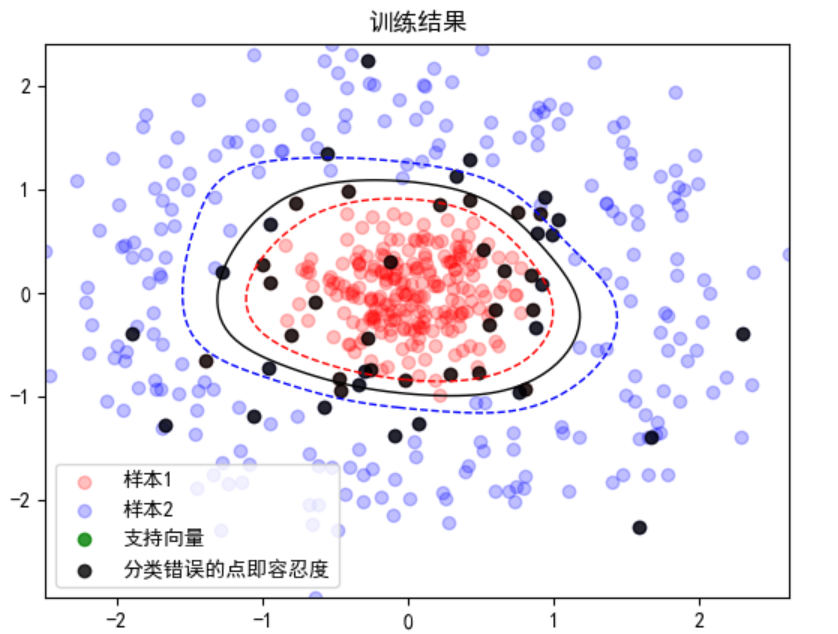
\includegraphics[width=0.8% 图片尺寸,可自行调节
			\textwidth]{figure10}% 图片名称(图片需与tex文件在同一文件夹)
			\caption{\fontsize{10pt}{15pt}\selectfont 仿真结果}% 图例
		\end{minipage}
	\end{figure}



\end{document}% 结束文档编辑,后面写啥都编译不出来